\chapter{Diseño técnico}

\section{Listado de historias de usuario (Backlog)}

\section{Historias de usuario}

\section{Metodologías y tecnologías de base que podrían usarse}

\subsection{Lenguaje de programación}
Se plantean los siguientes lenguajes de alto nivel, que disponen de frameworks implementados para crear un bot de Telegram:

\begin{itemize}
    \item \textbf{JavaScript}: es un lenguaje compilado en tiempo de ejecución, con tipado dinámico y multi-paradigma, soportando programación orientada a objetos, funcional, imperativa y dirigida por eventos\cite{wiki:JavaScript}. Se conforma al estándar ``ECMAScript'', y es una de las tecnologías centrales de la World Wide Web: el 98\% de los sitios web lo usan en el lado del cliente\cite{javascriptUsage}, y desde el surgimiento de Node.js es una tecnología en auge para servidores.
    \item \textbf{TypeScript} (\url{https://www.typescriptlang.org/}): es un superconjunto de JavaScript que añade sintaxis para tipos estáticos, y a través de un compilador genera código JavaScript\cite{typescriptWeb}. El añadido de tipos estáticos permite detectar errores de forma más temprana y agilizar la escritura de código gracias al autocompletado. Por otro lado, la adición de tipos es un tiempo extra empleado por el programador, por lo que debe analizarse si es conveniente su uso o no.
    \item \textbf{Python} (\url{https://www.python.org/}): es un lenguaje interpretado, interactivo y principalmente orientado a objetos, aunque soporta otros paradigmas como el funcional o el procedimental\cite{pythonFAQGeneral}. Es muy usado en el campo de la computación científica y la inteligencia artificial. Su uso en el desarrollo web se ha extendido para el lado del servidor con la aparición de frameworks como Django (\url{https://www.djangoproject.com/}) o Flask (\url{https://flask.palletsprojects.com/}).
    \item \textbf{PHP} (\url{https://www.php.net/}): es un lenguaje interpretado usado principalmente para desarrollo web en el lado del servidor, cuya principal característica es que puede ser embebido en HTML, de forma que cada ``trozo de PHP'' se ejecuta para intercambiarse por HTML. Sin embargo su uso ha cambiado en los últimos años, dando lugar a frameworks como Symphony (\url{https://symfony.com/}) o Laravel (\url{https://laravel.com/}) basados en la arquitectura Modelo-vista-controlador.
\end{itemize}

Se proporciona una tabla comparativa entre los lenguajes, la tabla \ref{tab:comparacionLenguajes}.

\begin{table}
\begin{minipage}{\textwidth}
\begin{tabularx}{\textwidth}{|l|X|X|X|X|}
\hline
   & JavaScript                       & TypeScript             & Python                    & PHP                       \\
\hline
Tipo                                                & Compilado en tiempo de ejecución & Compilado a JavaScript & Interpretado              & Interpretado              \\
\hline
Tipado estático                                     & No                               & Sí                     & Poco estricto, y poco uso & Poco estricto, y poco uso \\
\hline
Coste\footnote{Aprendizaje necesario por parte del autor para poder implementar el proyecto}                                & Nulo                             & Bajo                   & Medio                     & Medio                     \\
\hline
Popularidad\footnote{\url{https://survey.stackoverflow.co/2022/}} & 65.36\%                          & 34.83\%                & 48.07\%                   & 20.87\%                   \\
\hline
Comunidad \footnote{Preguntas totales en stackoverflow: \url{https://stackoverflow.com/tags}}      & 2432281                          & 196707                 & 2035248                   & 1447104               \\
\hline
\end{tabularx}
\end{minipage}
\caption{Comparación de lenguajes de programación}\label{tab:comparacionLenguajes}
\end{table}


\subsection{Framework para el desarrollo del bot}

Existen diversas bibliotecas que ayudan a crear un bot, de forma que no haya que escribir todo el código desde cero para interaccionar con la API de Telegram, siguiendo el principio ``Don't Reinvent the Wheel'' (``No reinventes la rueda'') para también ahorrar presupuesto.

Las opciones que se analizan son:

\begin{itemize}
    \item \textbf{Telegraf} (\url{https://telegraf.js.org/}): biblioteca desarrollada inicialmente para JavaScript, migrada en la versión 4 dando soporte a TypeScript. No dispone de documentación guiada, y la migración a la versión 4 trajo consigo más complejidad de uso. Está inspirada el sistema de middleware de Express.\footnote{\url{https://expressjs.com/es/guide/using-middleware.html}}
    \item \textbf{grammY} (\url{https://grammy.dev/}): biblioteca desarrollada desde un inicio para TypeScript (aunque se puede usar con JavaScript). Está inspirada en telegraf y fue creada desde cero por uno de los antiguos mantenedores de Telegraf como única forma de resolver sus mayores inconvenientes\footnote{\url{https://github.com/telegraf/telegraf/discussions/1526}}. Dispone de una completa documentación con guías para cada uno de los conceptos importantes.
    \item \textbf{node-telegram-bot-api} (\url{https://github.com/yagop/node-telegram-bot-api}): biblioteca ligera para interactuar con la API de Telegram, diseñada para Node.js, y no implementa un sistema de middleware.
    \item \textbf{python-telegram-bot} (\url{https://python-telegram-bot.org/}): biblioteca para Python que provee clases de alto nivel como capa de abstracción sobre la API de Telegram.
\end{itemize}

La tabla \ref{tab:comparacionFrameworks} compara los distintos frameworks.

\begin{table}
\begin{minipage}{\textwidth}
\begin{tabularx}{\textwidth}{|l|X|X|X|X|}
\hline
& telegraf & grammY & node-telegram-bot-api & python-telegram-bot \\
\hline
Lenguaje & JavaScript & Typescript & JavaScript & Python \\
\hline
Documentación & Autogenerada, solo API & Completa, numerosos tutoriales & Básica & Autogenerada, solo API \\
\hline
\makecell[l]{Versión API \\Telegram} & 6.2 & 6.2 & 6.2 & 6.2 \\
\hline
Popularidad\footnote{Estrellas en GitHub a 7 de octubre de 2022} & 6.1k & 663 & 6.5k & 19.8k \\
\hline
\end{tabularx}
\end{minipage}
\caption{Comparación de frameworks para creación de bots de Telegram}\label{tab:comparacionFrameworks}
\end{table}

\subsection{Base de datos}

La base de datos es ``una colección compartida de datos lógicamente relacionados, junto con una descripción de estos datos, que están diseñados para satisfacer las necesidades de información de una organización''.\cite{alma991009264529704990}

Por otra parte, el sistema gestor de base de datos (SGBD) es ``un sistema software que permite a los usuarios definir, mantener, crear y controlar el acceso a la base de datos.\cite{alma991009264529704990}

Necesitaremos estas herramientas ya que buscamos un sistema que guarde datos de manera persistente y poder recuperarlos y actualizarlos en cualquier momento.

Se analizan alternativas para bases de datos relacionales, basadas en el concepto matemático de relación, representado por tablas\cite{alma991009264529704990}; y también para bases de datos no relacionales documentales.

\begin{itemize}
    \item Para bases de datos relacionales:
    \begin{itemize}
        \item PostgreSQL (\url{https://www.postgresql.org/}): es un SGBD de código abierto y centrado en la escabilidad.
        \item MySQL (\url{https://www.mysql.com/}): es un SGDB de código abierto desarrollado por Oracle.
        \item MariaDB (\url{https://mariadb.org/}): es un SGDB de código abierto creado por desarrolladores de MySQL como respuesta a la adquisición por parte de Oracle, y con características muy parecidas.
    \end{itemize}
    \item Para bases de datos no relacionales:
    \begin{itemize}
        \item MongoDB (\url{https://www.mongodb.com/}): SGDB de código disponible (no necesariamente de código abierto, por usar una licencia SSPL.\cite{ssplLicense}
        \item Firestore (\url{https://firebase.google.com/docs/firestore}): incluido en la suite de servicios ``Firebase'' de Google destinada a la gestión rápida y centralizada de aplicaciones.
    \end{itemize}
\end{itemize}


% Puesto que las diferencias son pequeñas entre las opciones de base de datos relacional y la documentación de Prisma está mayormente basada en PostgreSQL, se escoge esta opción.

%\subsection{ORM}
%\begin{itemize}
%    \item TypeORM
%    \item Sequelize
%    \item Prisma
%\end{itemize}

\subsection{Almacenamiento de archivos}
\begin{itemize}
    \item Amazon S3
    \item DigitalOcean Spaces
    \item Google Cloud Storage / Firestore Storage
\end{itemize}

\subsection{IDE}
\begin{itemize}
    \item VSCode
    \item JetBrains
\end{itemize}

%\subsection{Gestor de paquetes}
%\begin{itemize}
%    \item npm
%    \item yarn
%    \item pnpm
%\end{itemize}

\subsection{Documentación}
\begin{itemize}
    \item Docusaurus
    \item GitBook
    \item VuePress
\end{itemize}


\section{Modelo de la base de datos}

\section{Arquitectura de Mordente}

Expliquemos la arquitectura utilizada en dos pasos:

\subsection{Arquitectura entre puntos}

Con la arquitectura entre puntos nos referimos a la visualización a alto nivel de las distintas partes físicas necesarias para que nuestra herramienta funcione.

En nuestro caso, existen tres partes claramente diferenciadas:

\begin{itemize}
    \item \textbf{El dispositivo del usuario}, o también llamado cliente. Tiene instalada la aplicación de Telegram, y se comunica bidireccionalmente con los servidores de Telegram para enviar y recibir mensajes.
    \item \textbf{Los servidores de Telegram}. Actúan como intermediarios entre distintos usuarios, así como entre los usuarios y nuestro bot.
    \item \textbf{El bot}. Es un programa que se comunica con los servidores de Telegram para enviar y recibir mensajes, tal y como los clientes, aunque con ciertas diferencias de funcionamiento con los clientes. Este programa puede estar alojado en cualquier ordenador, y en nuestro caso estará alojado en un servidor privado virtual.
\end{itemize}

Esta arquitectura está representada en la figura \ref{fig:arquitecturaPuntos}.

\begin{figure}[h]
\centering
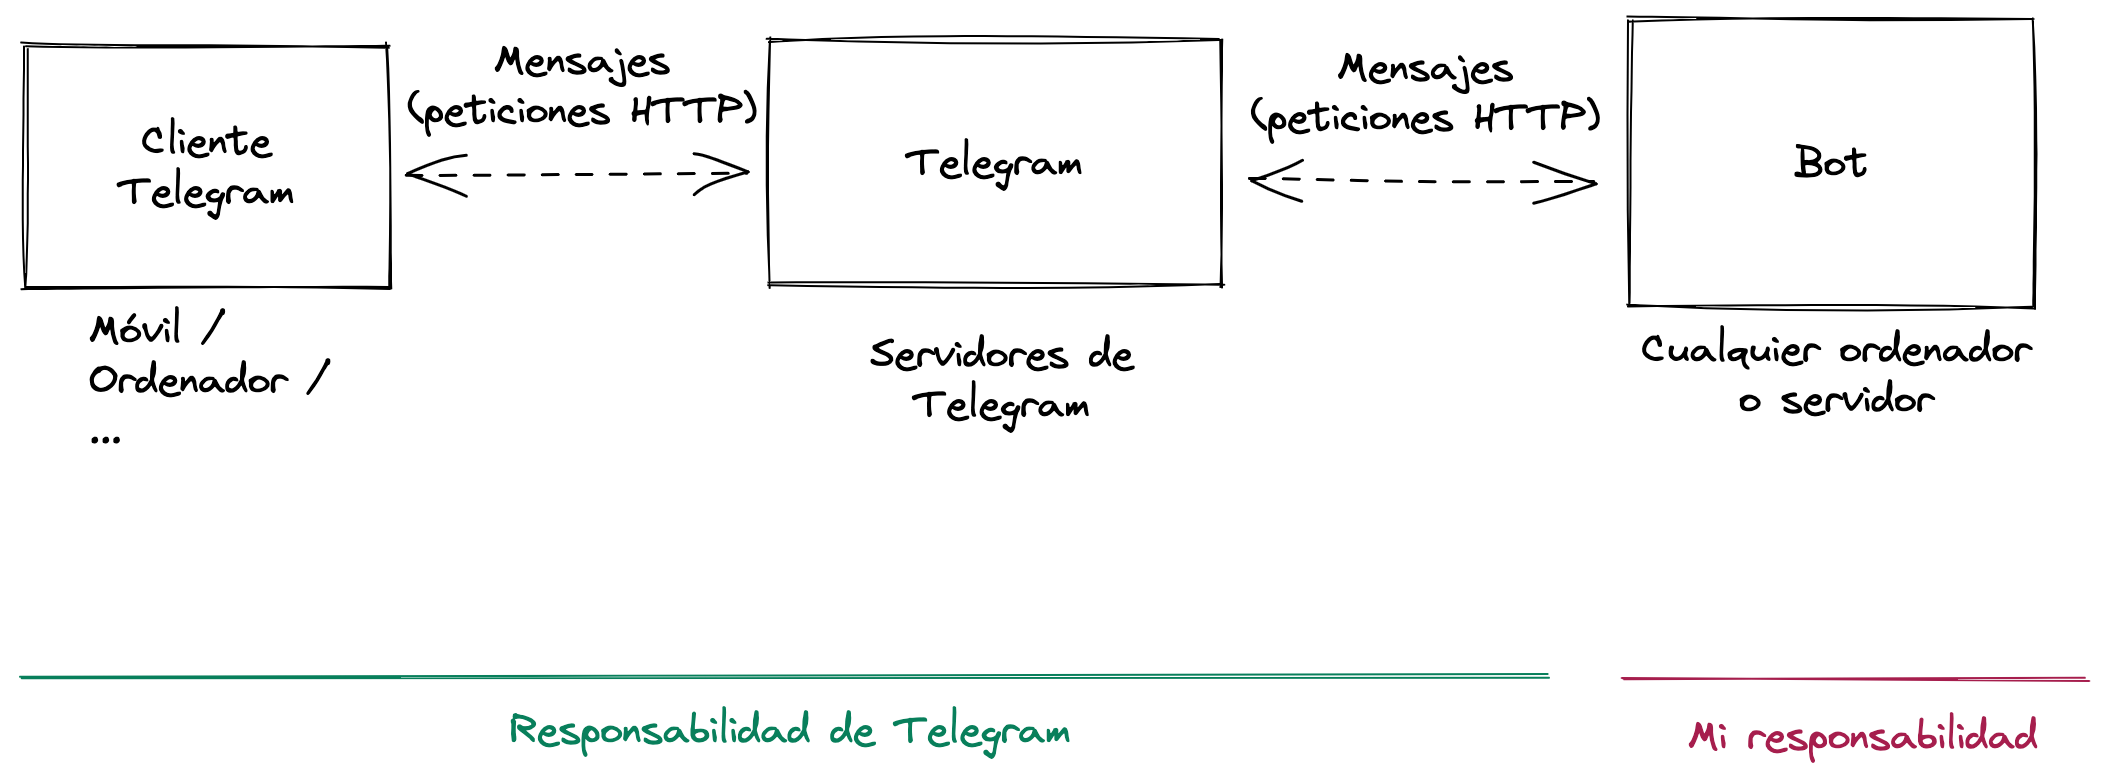
\includegraphics[width=1\textwidth]{imagenes/disenyo_tecnico/arquitectura_puntos.png}
\caption{Arquitectura entre puntos}
\label{fig:arquitecturaPuntos}
\end{figure}

Es importante entender que la única responsabilidad que nos corresponde a nosotros es la de desarrollar la última parte: el bot. El cliente y los servidores de Telegram son partes externas fuera de nuestra responsabilidad, lo cual es una de las ventajas de desarrollar un servicio de este tipo.


% VPS   <->   Telegram API   <->    Telegram Client


\subsection{Arquitectura entre servicios}

Para la funcionalidad que necesitamos, el bot debe estar compuesto por varios microservicios a su vez: 

\begin{itemize}
    \item \textbf{El propio bot:} es el microservicio donde implementaremos la comunicación con los servidores de Telegram para recibir mensajes, procesarlos y responderlos adecuadamente.
    \item El bot realiza peticiones a una \textbf{base de datos} donde almacenaremos de forma persistente los datos de los usuarios. Esto garantizará que no perdamos información cuando el bot se reinicie.
    \item Opcionalmente, podremos añadir un microservicio encargado de realizar una \textbf{copia de seguridad} periódica de la base de datos.
    \item Por otro lado tendremos un servicio de \textbf{almacenamiento de archivos} para guardar las copias de seguridad y otros archivos (en nuestro caso, las partituras).
\end{itemize}

En la figura \ref{fig:arquitecturaServicios} se puede visualizar la arquitectura entre los distintos servicios.

\begin{figure}[h]
\centering
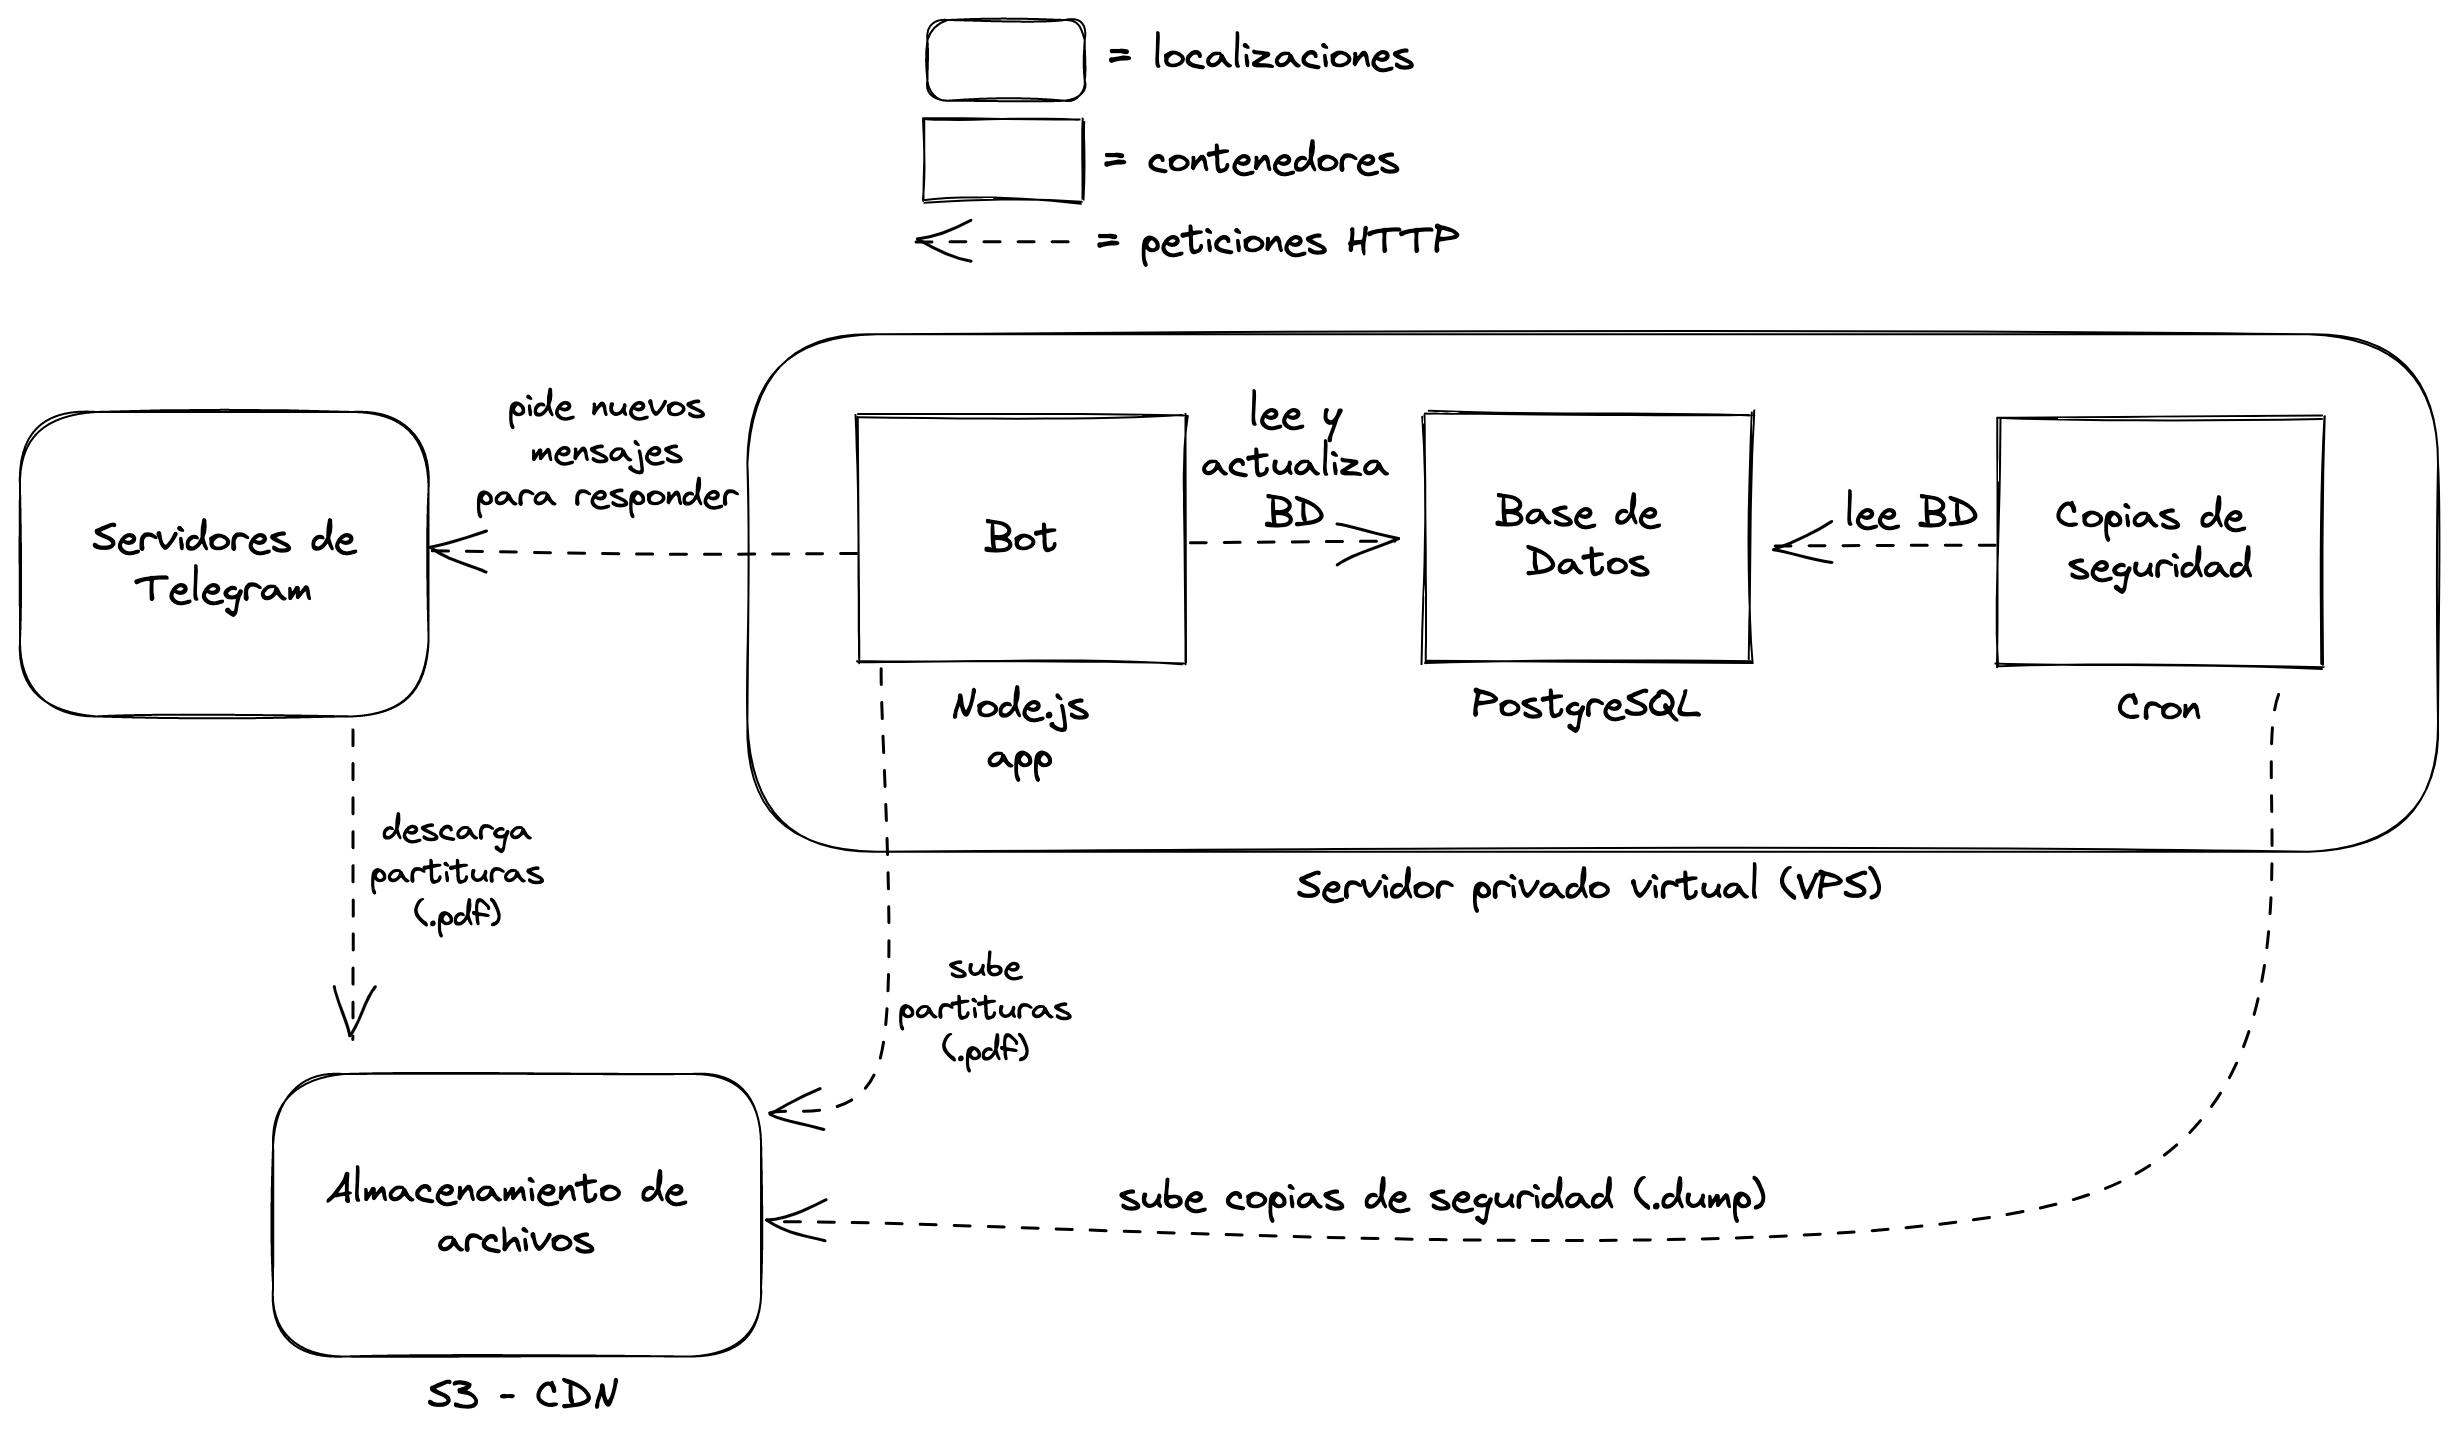
\includegraphics[width=\textwidth]{imagenes/disenyo_tecnico/arquitectura_servicios.png}
\caption{Arquitectura entre servicios}
\label{fig:arquitecturaServicios}
\end{figure}

\subsubsection{Localización de los servicios}

Con respecto a dónde disponer los distintos servicios, existen al menos dos opciones: una es alojarlos en el propio servidor que gestionaremos nosotros y cuyos microservicios podremos levantar en un solo paso usando \textit{Docker Compose}, y otra es utilizar servicios auto-gestionados por plataformas externas. Hagamos una reflexión para cada uno de los servicios:

\begin{itemize}
    \item El \textbf{bot} puede estar en un servidor propio o en un servicio gestionado, ambas opciones son válidas. La ventaja de tenerlo en el servidor propio será la mayor cercanía posible con la base de datos, resultando en una mayor velocidad de respuesta. La ventaja de utilizar un servicio gestionado es la mayor facilidad de escalado, sin embargo esto no es algo prioritario en la primera fase de desarrollo.
    \item Casi todos los proveedores de servicios en la nube ofrecen \textbf{bases de datos} gestionadas\footnote{Ejemplos: Digital Ocean Managed Databases, Heroku Postgres, Firebase Cloud Firestore...}, aunque siempre es conveniente que el bot y la base de datos se encuentren físicamente cercanos para reducir la latencia de las frecuentes consultas. Es por ello y porque no se prevé una gran cantidad de información almacenada durante el periodo inicial que optaremos por alojar la base de datos dentro de nuestro servidor, al igual que el bot.
    \item El \textbf{almacenamiento de archivos} siempre se suele delegar a un servicio externo gestionado. La mayor ventaja de esta aproximación es la disponibilidad de una CDN (\textit{Content Delivery Network}, o Red de Entrega de Contenidos). Gracias a esta red tendremos un conjunto de servidores distribuidos geográficamente que pueden entregar rápidamente el contenido. Además, usar un servicio fuera de nuestro servidor garantiza que podamos realizar copias de seguridad de la base de datos que no se pierdan si el servidor se rompe por cualquier causa.
\end{itemize}


\subsubsection{Entorno de producción y de desarrollo}

Es importante tener en cuenta también que esta configuración puede variar dependiendo de si nos encontramos en el entorno de desarrollo o de producción. En nuestro caso, el servicio de copias de seguridad no existirá en el entorno de desarrollo. 

Además, tendremos dos réplicas (una de producción y otra de desarrollo) del bot, la base de datos y el almacenamiento de archivos para que las pruebas no afecten en ningún caso a los datos de los usuarios reales.

\section{Seguridad}

Se intentará maximizar la seguridad de la aplicación gracias a los siguientes puntos:

\begin{itemize}
    \item Los contenedores de Docker utilizados en el servidor están completamente aislados de la red excepto en los puertos que configuremos manualmente. En nuestro caso, el bot podrá conectarse a la base de datos pero ninguno de los contenedores tendrá puertos expuestos al exterior que pudieran ser usados por atacantes.
    \item Gracias al punto anterior, los ataques de denegación de servicio (DDoS) no son un riesgo. Además el servidor tendrá un Firewall configurado.
    \item El uso de herramientas \textit{open-source} como Prisma para hacer las consultas a la base de datos en lugar de realizarlas manualmente con código SQL disminuye al máximo la posibilidad de Inyecciones SQL.
    \item La inyección de código al servidor no es posible ya que no se ejecuta ningún código enviado por el cliente, y por otro lado el cliente es responsabilidad de Telegram.
    \item Se añadirán métodos que permitan detectar automáticamente las vulnerabilidades introducidas por dependencias externas. Como el repositorio estará alojado en GitHub, se propone el uso de \textit{Dependabot}\footnote{\url{https://docs.github.com/es/code-security/dependabot}}.
\end{itemize}


% VPS:

% Telegram API   <->   | app | Postgre | backup |

% Contenedores aislados -> total seguridad
